\newpage
\subsection{Fabric interface}

\begin{figure}[ht]
  \begin{center}
    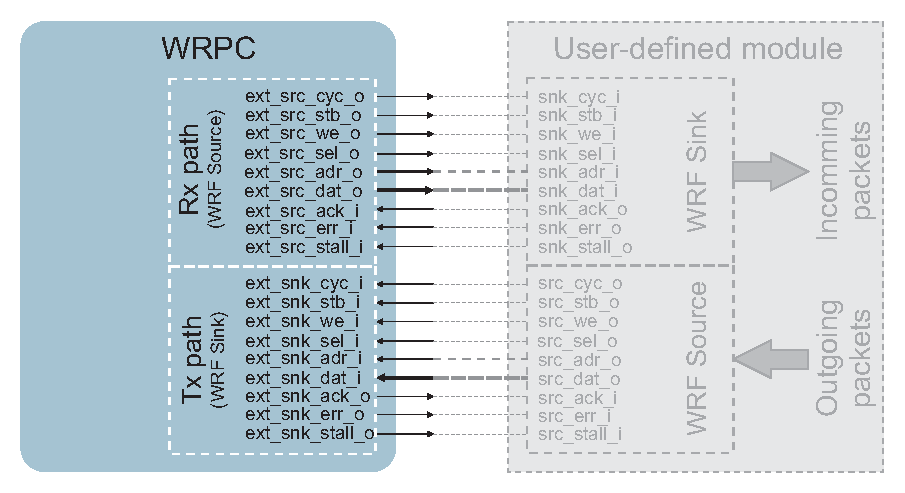
\includegraphics[width=\textwidth]{fig/wrpc_fabric.pdf}
    \caption{WR Fabric interface}
  \end{center}
\end{figure}

The Fabric interface is used for sending and receiving Ethernet frames. It consists 
of two pipelined Wishbone interfaces operating independently: 
\begin{itemize}
  \item \emph{WRF Source}: pipelined Wishbone Master, passes all the Ethernet frames
    received from a physical link to WRF Sink interface implemented in a
    user-defined module.
  \item \emph{WRF Sink}: pipelined Wishbone Slave, receives Ethernet frames from
    the WRF Source implemented in the user-defined module, and sends them to a
    physical link.
\end{itemize}
Each of the Pipelined Wishbone buses being part of WR Fabric interface consist
of the following signals:
\begin{center}
  \begin{tabular}{|l|l|l|p{10cm}|}
    \hline
    {\bf Signal name} & {\bf size} & {\bf direction} & {\bf description} \\
    \hline
    \hline \texttt{adr} & 2 & Source $\rightarrow$ Sink & defines what kind of data is actually available on data bus\\
    \hline \texttt{dat} & 16 & Source $\rightarrow$ Sink & data bus \\
    \hline \texttt{sel} & 2 & Source $\rightarrow$ Sink & byte/word select (single
    byte can be transmitted only as the last data word of the frame)\\
    \hline \texttt{cyc} & 1 & Source $\rightarrow$ Sink &  indicates a valid bus cycle\\
    \hline \texttt{stb} & 1 & Source $\rightarrow$ Sink &  indicates a valid data
    transfer cycle\\
    \hline \texttt{we}  & 1 & Source $\rightarrow$ Sink & write enable (always high)\\
    \hline \texttt{ack} & 1 & Sink $\rightarrow$ Source & data acknowledge\\
    \hline \texttt{err} & 1 & Sink $\rightarrow$ Source & Sink error indicator\\
    \hline \texttt{stall} & 1 & Sink $\rightarrow$ Source & used by Sink for flow control\\
    \hline
  \end{tabular}
\end{center}

For a more precise description of the Pipelined Wishbone signals please check the
Wishbone B4 Specification \cite{wb_spec}.\\

{\bf Address bus} can have one of the following values:
\begin{center}
\begin{tabular}{|c|l|}
  \hline {\bf decimal value} & {\bf meaning of data word on data bus}\\
  \hline
  \emph{0} & regular data (packet header and payload)\\
  \emph{1} & OOB (Out-of-band) data\\
  \emph{2} & status word\\
  \hline
\end{tabular}
\end{center}

{\bf Status word} (sent when the value of the address bus is \emph{2}) contains
the information about Ethernet frame's structure and type:
\begin{figure}[ht]
  \begin{center}
    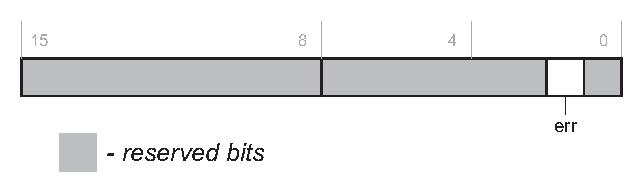
\includegraphics[width=.6\textwidth]{fig/basic_wrf_status.pdf}
    \caption{Simplified status word format}
  \end{center}
\end{figure}

\begin{itemize}
  \item[] \emph{err} - if \emph{1}, the frame contains an error. It may occur when
    the size of Ethernet frame is too small or it contains invalid CRC checksum.
\end{itemize}
\begin{figure}[hbt]
  \begin{center}
    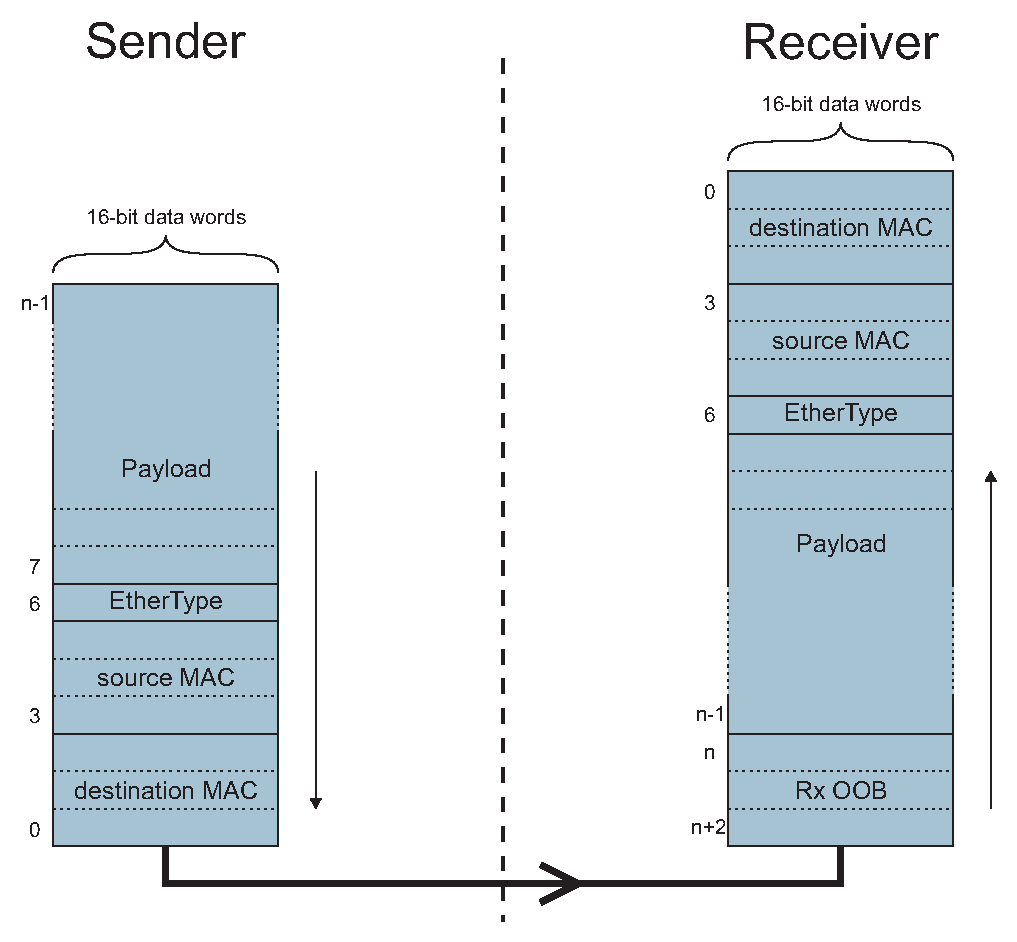
\includegraphics[width=.6\textwidth]{fig/basic_wrf_data.pdf}
    \caption{Data words that make the Ethernet frame}
    \label{fig:fabric:simple_data}
  \end{center}
\end{figure}

Figure \ref{fig:fabric:simple_data} presents data words fed to the WRF
data bus by the sender and the information got at the receiving side. Please
note that the CRC checksum is calculated and inserted automatically inside the
WRPC and user-defined module doesn't care about it. The Ethernet frame received
from the WR Fabric interface may contain additional OOB data suffixed. It has to
be received (acknowledged) by the user-defined module, but can be simply discarded.

\subsubsection{Examples}
Figure \ref{fig:fabric:simple_tx} shows a very simple WR Fabric cycle. The WRF
Source of user-defined module sends there an Ethernet frame containing even
number of bytes.

\begin{figure}[ht]
  \begin{center}
    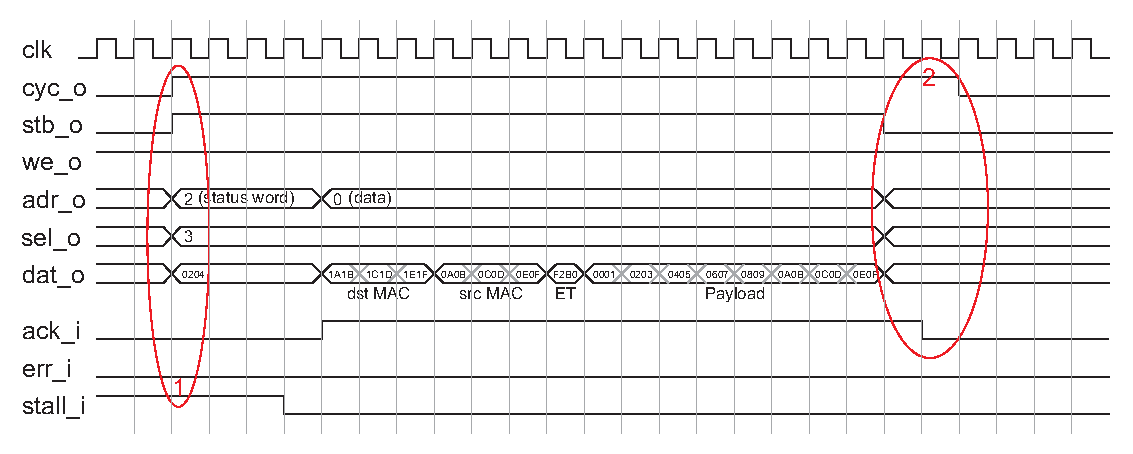
\includegraphics[width=\textwidth]{fig/basic_wrf_cycle_simple.pdf}
    \caption{Simple WR Fabric cycle - user-defined module sending packet}
    \label{fig:fabric:simple_tx}
  \end{center}
\end{figure}

\begin{enumerate}
  \item The WRF Source in user-defined module starts the cycle by asserting
    \emph{cyc\_o}, \emph{stb\_o} and putting a status word to the data bus.
    However, since WRF Sink set \emph{stall} signal to active state, Source has
    to wait until Sink is ready to receive data.
  \item After the last word is transmitted, the WRF Source sets \emph{stb\_o} back
    to \emph{0}, but waits until Sink acknowledges all the words transmitted in
    the cycle (\emph{ack\_i} line). The cycle ends when \emph{cyc\_o} goes back
    to the low state.
\end{enumerate}

Figure \ref{fig:fabric:sel} shows again a very simple WR Fabric cycle where
user-defined WRF Source sends an Ethernet frame to the WRPC. This time though,
the frame contains odd number of bytes, therefore the \emph{sel} line is used to
signal this fact to WRF Sink inside the WRPC (1).

\begin{figure}[ht]
  \begin{center}
    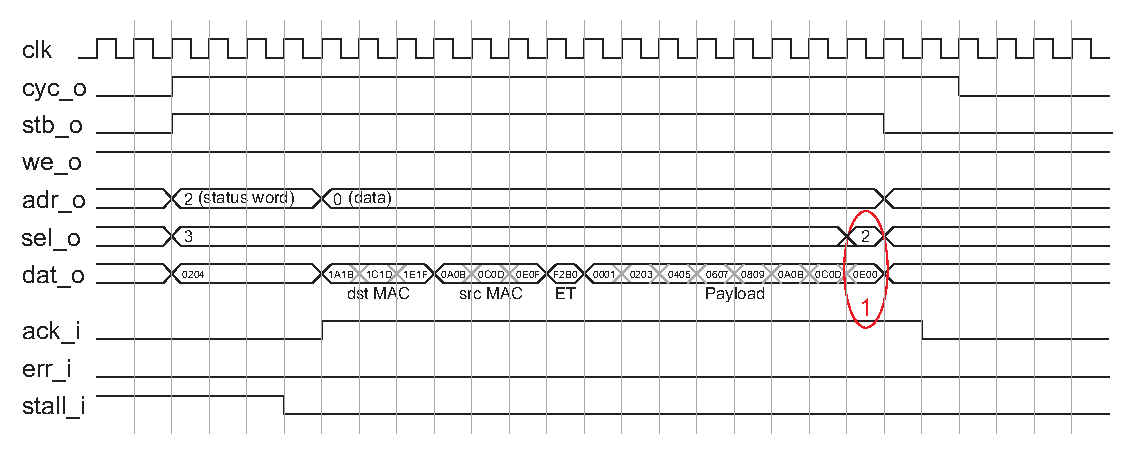
\includegraphics[width=\textwidth]{fig/basic_wrf_cycle_sel.pdf}
    \caption{Simple WR Fabric cycle - user-defined module sending packet(odd
    number of bytes in the payload)}
    \label{fig:fabric:sel}
  \end{center}
\end{figure}

Figure \ref{fig:fabric:cyc} presents more complicated Fabric cycle where an
Ethernet frame is received from WRF Source in the WRPC (output signals in the
diagram are driven by WRF Source on the WRPC side): 
\begin{figure}[ht]
  \begin{center}
    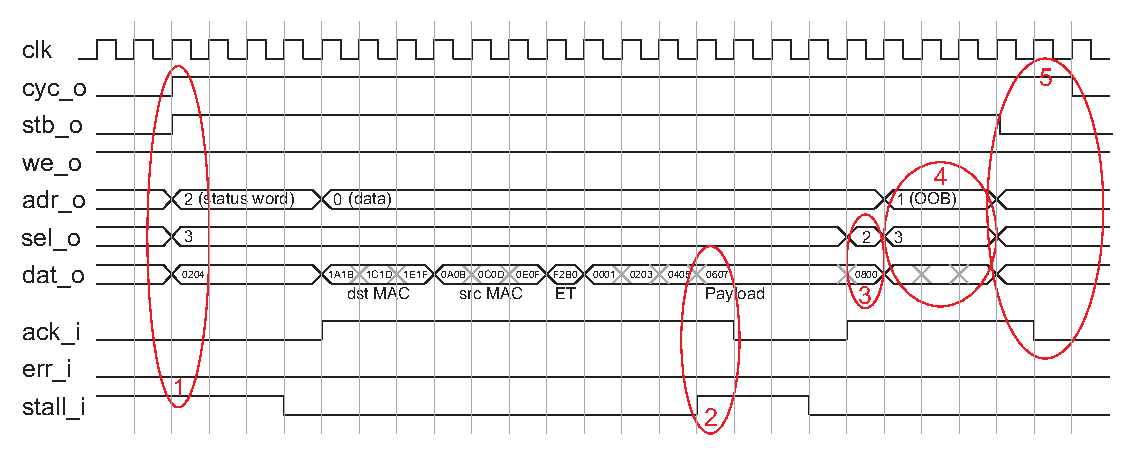
\includegraphics[width=\textwidth]{fig/basic_wrf_cycle.pdf}
    \caption{WR Fabric cycle}
    \label{fig:fabric:cyc}
  \end{center}
\end{figure}
\begin{enumerate}
  \item The WRF Source starts the cycle by asserting \emph{cyc\_o}, \emph{stb\_o}
    and putting a status word to the data bus. However, since WRF Sink set 
    \emph{stall} signal to active state, Source has to wait until Sink is ready
    to receive data.
  \item While the payload of the Ethernet frame is being transmitted, Sink
    stalls the cycle. The WRF Source pauses the transmission until Sink becomes
    ready to process the rest of the data. During that time \emph{stb\_o} has to
    remain in a high state.
  \item The Ethernet frame contains an odd number of bytes, so only half of last
    word of payload carries a valid data. \emph{Sel\_o} is used to signal this
    fact to WRF Sink.
  \item After the whole payload is transmitted, Source may additionally sent Rx
    OOB data. It contains some internal WRPC data that should be acknowledged
    by Sink, but discarded in the user's module.
  \item After the last word is transmitted, the WRF Source sets \emph{stb\_o} back
    to \emph{0}, but waits until Sink acknowledges all the words transmitted in
    the cycle (\emph{ack\_i} line). The cycle ends when \emph{cyc\_o} goes back
    to the low state.
\end{enumerate}

WRF Sink can use the \emph{stall} line to pause the frame transmission if it cannot
process the flow of data coming from WRF Source. However, if some more serious
problem appears on the receiving side, the \emph{err} line can be used to
immediately break the cycle. This situation is presented in figure
\ref{fig:fabric:cycerr}:
\begin{figure}[ht]
  \begin{center}
    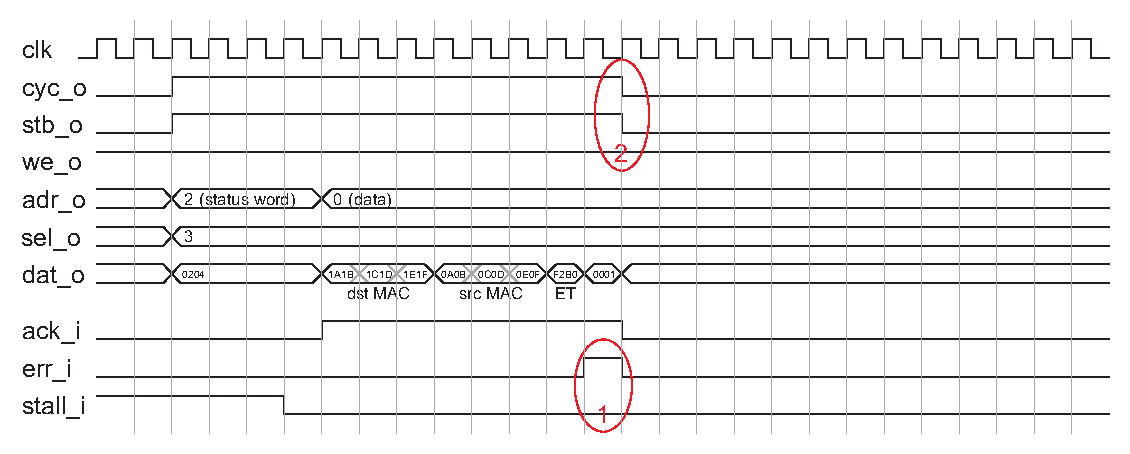
\includegraphics[width=\textwidth]{fig/basic_wrf_cycle_err.pdf}
    \caption{WR Fabric cycle interrupted with an error line}
    \label{fig:fabric:cycerr}
  \end{center}
\end{figure}
\begin{enumerate}
  \item WRF Sink wants to break a bus cycle, so it drives \emph{err\_i} high.
  \item WRF Source breaks the cycle immediately after receiving an error indicator
    from the WRF Sink.
\end{enumerate}

\subsubsection{SystemVerilog model}
The SystemVerilog simulation model of the WR Fabric interface (both WRF Source and 
WRF Sink) can be found in the \emph{wr-cores} git repository
(git://ohwr.org/hdl-core-lib/wr-cores.git) and consists of the files:
\begin{itemize}
  \item \emph{sim/if\_wb\_master.svh}
  \item \emph{sim/if\_wb\_slave.svh}
  \item \emph{sim/wb\_packet\_source.svh}
  \item \emph{sim/wb\_packet\_sink.svh}
\end{itemize}

The testbench example using the simulation model of WR Fabric interface can
be found in the zip archive attached to this documentation.
